\documentclass{beamer}
\usepackage[utf8]{inputenc}
\usepackage[T1]{fontenc}
\usepackage{graphicx}
\usepackage{grffile}
\usepackage{longtable}
\usepackage{wrapfig}
\usepackage{rotating}
\usepackage[normalem]{ulem}
\usepackage{amsmath}
\usepackage{textcomp}
\usepackage{amssymb}
\usepackage{capt-of}
\usepackage{hyperref}
\newcommand{\inlinelatex}[1]{#1}
\usetheme{Madrid}
\setbeamertemplate{frametitle continuation} {}
\title[CMP223]{Performance and Cost-Aware in HPC: A Network Interconnect Impact Assessment}
\author[Anderson M.M]{\large{Anderson M. Maliszewski}}
\institute[UFRGS]{\small{Parallel and Distributed Processing Group (GPPD)\\
Informatics Institute (INF)\\
Federal University of Rio Grande do Sul (UFRGS) \\Porto Alegre - Brazil}}
\date[11 December, 2019]{\large{CMP223 Computer System Performance Analysis (2019/2)\\
11 December, 2019}}
\logo{
\includegraphics[width=1.3cm,keepaspectratio]{SLIDES/logo/ufrgs.png}~~~~~~~~~~~~~~~~~~~~~~~~~~~~~~~~~~~~~~~~~~~~~~~~~~~~~~~~~~~~~~~~~~~~~
%\hspace{\dimexpr\paperwidth-5cm-1pt}%
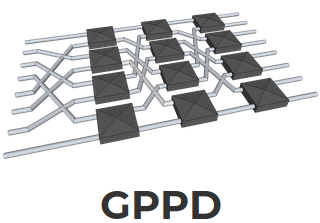
\includegraphics[width=1.3cm,keepaspectratio]{SLIDES/logo/GPPD-logo.png}~~~~~~~~~~~~~~~~~~~~~~~~~~~~~~~~~~~~~~~~~~~~~~~~~~~~~~~~~~~~~~~~~~~~~
%\hspace{\dimexpr\paperwidth-3cm-1pt}%

\includegraphics[width=1.5cm,keepaspectratio]{SLIDES/logo/inf-logo.png}%
}

\colorlet{beamer@blendedblue}{black}
\setbeamercolor{alerted text}{fg=orange}

\begin{document}
\maketitle
\logo{
\includegraphics[width=1.5cm]{SLIDES/logo/inf-logo.png}}
\begin{frame}{Introduction}
\vfill
Growing demand for computational power
\begin{itemize}
\item High Performace Computing (HPC)
\item Clusters and "as a Service" cloud models
\end{itemize}
\pause \vfill
Communication characteristics vary
\begin{itemize}
\item Specific proposal for parallel programs
\item Bandwidth and latency-sensitive
\end{itemize}
\pause \vfill
Network interconnection is directly related to performance losses
\begin{itemize}
\item High ṕerformance interconnects - InfiniBand
\end{itemize}
\end{frame}

\begin{frame}{Motivation}
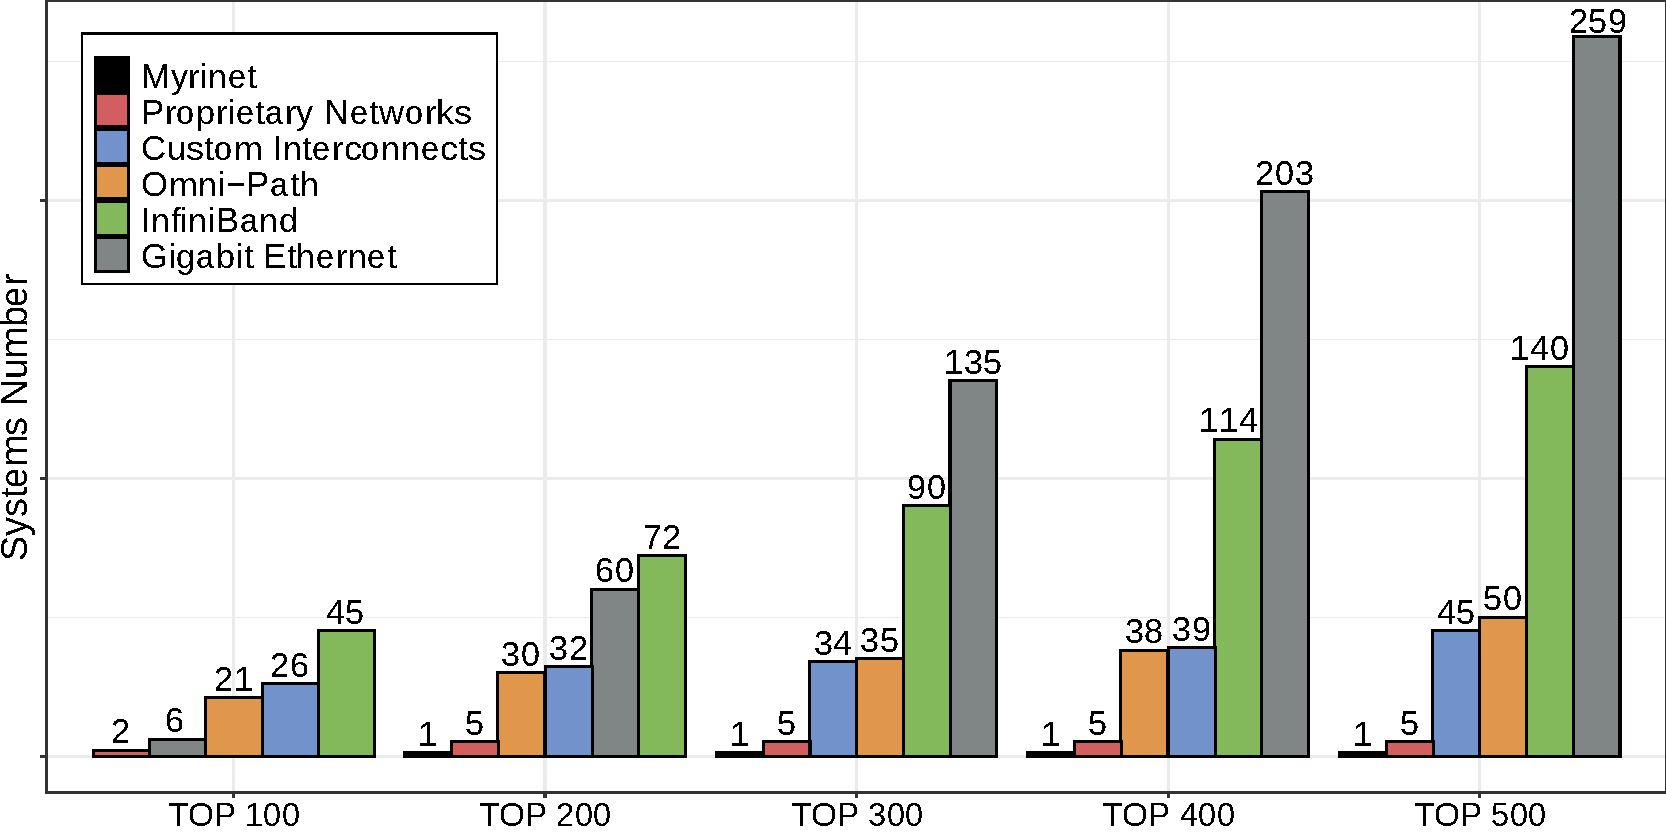
\includegraphics[width=\textwidth]{SLIDES/img/TOP500-5.pdf}
\end{frame}


\begin{frame}{Objective}
\vfill
Assess the impact of the \alert{network interconnection} on HPC applications regarding performance and cost execution

\pause \vfill
How do the \alert{communication characteristics} of applications influence their performance?

\pause \vfill
To answer these questions:

\pause \vfill
\begin{itemize}
    \item  Both \alert{InfiniBand (IB)} and \alert{Gigabit Ethernet (ETH)}, as well as \alert{IP-over-IB (IPoIB)} interconnections were evaluated using the same physical cluster of servers
\pause \vfill
    \item All applications are also profiled, in which their MPI operations were exposed.
\pause \vfill
    \item The cost was calculated using the Microsoft Azure instance pricing model, in which the instances have the same hardware, differing only by interconnection (IB and Ethernet)
\end{itemize}
\vfill
\end{frame}

\begin{frame}{Outline}
\vfill
\Large
\begin{itemize}
\item Methodology
\begin{itemize}
\item System
\item Testbed
\item Applications
\item Trace
\item Experimental Design
\item Reproducible Research
\end{itemize}
\end{itemize}
\begin{itemize}
\item Results
\end{itemize}
\begin{itemize}
\item Conclusion
\item Future Work
\end{itemize}
\end{frame}

\begin{frame}  [plain, noframenumbering]
\begin{block}{}
\begin{center}
\Huge{Methodology}
\end{center}
\end{block}
\end{frame}

\begin{frame}[noframenumbering, allowframebreaks]{System}
\vspace{-0.3cm}
\begin{center}
    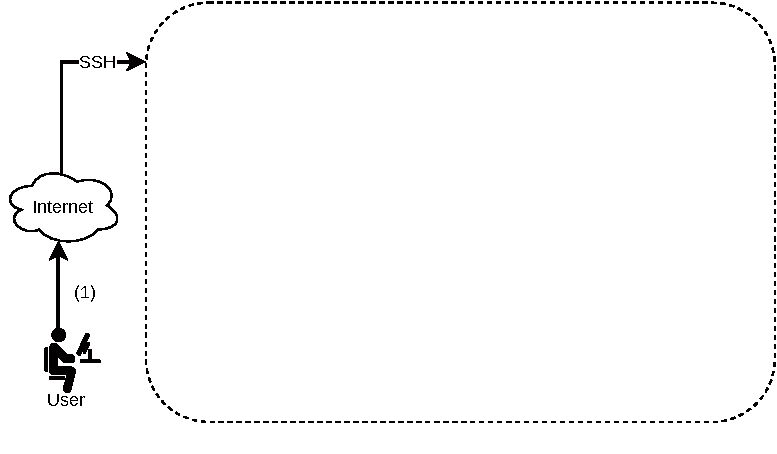
\includegraphics[scale=0.65]{SLIDES/img/System1.pdf}
\end{center}
    \begin{itemize}
    \item (1) User submits a job
    \item[~] 
    \item[~]
    \item[~] 
    \end{itemize}
    \framebreak
\begin{center}
    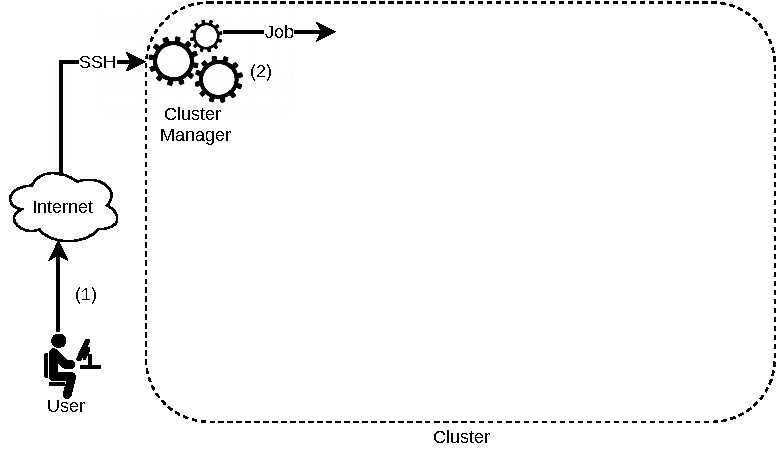
\includegraphics[scale=0.65]{SLIDES/img/System2.pdf}
\end{center}
    \begin{itemize}
    \item (1) User submits a job
    \item (2) Cluster manager allocates the nodes
    \item[~] 
    \item[~]
    \end{itemize}
    \framebreak
\begin{center}
    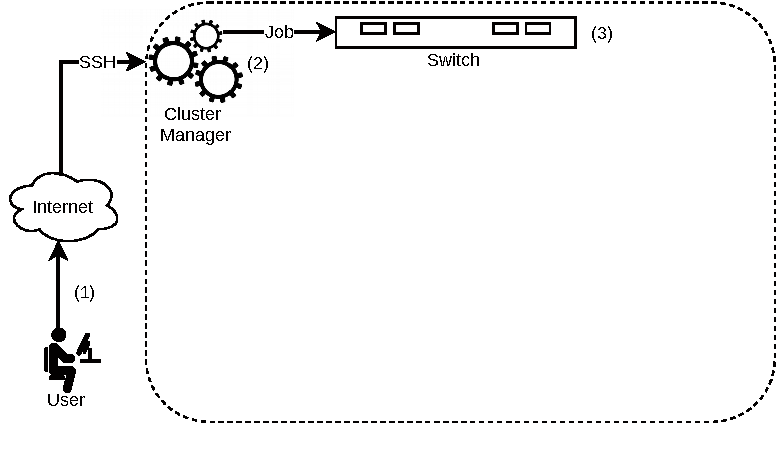
\includegraphics[scale=0.65]{SLIDES/img/System3.pdf}
\end{center}    
    \begin{itemize}
    \item (1) User submits a job
    \item (2) Cluster manager allocates the nodes
    \item (3) Job is passed to a switch
    \item[~]
    \end{itemize}
    \framebreak
\begin{center}
    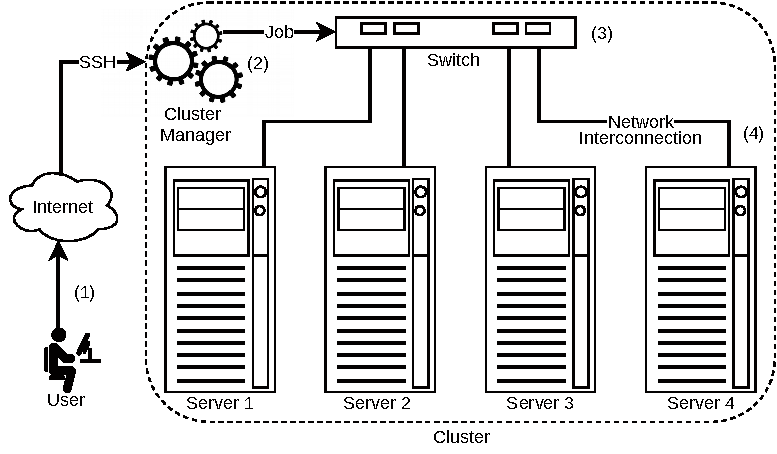
\includegraphics[scale=0.65]{SLIDES/img/System4.pdf}
\end{center}    
    \begin{itemize}
    \item (1) User submits a job
    \item (2) Cluster manager allocates the nodes
    \item (3) Job is passed to a switch
    \item (4) Switch acts as a central point of nodes communication
    \end{itemize}
\end{frame}

\begin{frame}{Testbed}
PCAD's Hype cluster \footnote{[1] http://gppd-hpc.inf.ufrgs.br/}
\begin{itemize}
\item 2 \texttimes{} Intel Xeon E5-2650 v3 (Q3'14) Haswell, 2.3 GHz
\item 20 cores (10 per CPU) with HT enabled resulting in 40 threads
\item 128 GB DDR4 RAM
\item Gigabit Ethernet and InfiniBand FDR interconnects
\item Ubuntu Server 18.04.01
\vfill
\end{itemize}
\vfill
\end{frame}

\begin{frame}{Applications}
Network characterization (Bandwidth and Latency)
    \begin{itemize}
        \item Intel MPI Benchmarks 
        \begin{itemize}
            \item PingPong
        \end{itemize}
    \end{itemize}
    \pause \vfill
Synthetic applications performance
    \begin{itemize}
        \item NPB 3.4 MPI
        \begin{itemize}
            \item BT, CG, EP, FT, IS, LU, MG, and SP
            \item Input class D
        \pause \vfill
        \end{itemize}
        \item ImbBench 
        \begin{itemize}
            \item CPU and Memory
            \item 8 Levels of Imbalance
        \end{itemize}
        \end{itemize}
        \pause \vfill
Real application performance
    \begin{itemize}
        \item Alya
    \end{itemize}
\end{frame}

\begin{frame}{Trace}
To trace the applications we used: 
    \pause \vfill
    \begin{itemize}
        \item Score-P 6.0
        \begin{itemize}
            \item Responsible for introducing the code instrumentation
        \end{itemize}
    \pause \vfill
        \item Akypuera
        \begin{itemize}
            \item \texttt{otf22paje}
                \begin{itemize}
                    \item Convert the OTF2 output to TRACE file
                \end{itemize}
        \end{itemize}
    \pause \vfill
        \item PajeNG
        \begin{itemize}
            \item \texttt{pj\_dump}
                \begin{itemize}
                    \item Convert the TRACE file to a CSV to be analysed in R
                \end{itemize}
        \end{itemize}
    \end{itemize}
\end{frame}


\begin{frame}{Experimental Design}
\vfill
Was created using the DoE.base library in R
\begin{itemize}
    \item Follows a full factorial design
    \item Two levels for each execution
 \begin{itemize}
\item Application: \alert{BT}, \alert{EP}, \alert{CG}, \alert{MG}, \alert{LU}, \alert{SP}, \alert{IS}, \alert{FT}, \alert{IMB\_Memory}, \alert{IMB\_CPU}, \alert{PinPong}, and \alert{Alya}
\item Network Interface: \alert{Gigabit Ethernet}, \alert{InfiniBand}, and \alert{IP-over-IB}
\end{itemize}
    \item 30 randomized replications
   \end{itemize}
N = (12 applications) \texttimes{} (3 interconnections) \texttimes{} (30 replications) = 1080 experiments\footnote{In the characterization execution the PingPong application was not executed and only one replication was performed, totaling in N = (11 applications) \texttimes{} (3 interconnections) = 33 experiments}   
\vfill
\end{frame}

\begin{frame}{Reproducible Research}
\vfill
Execution scripts
\begin{itemize}
    \item No user interaction
    \item 
    \item Collect system information
    \item Download all softwares/applications
    \item Compile
    \item Execute and collect the results
\end{itemize}

Org and Emacs
\begin{itemize}
    \item LabBook
    \begin{itemize}
        \item How to
    \end{itemize}
    \item R Blocks of code
\end{itemize}
\end{frame}


\begin{frame} [plain, noframenumbering]
\begin{block}{}
\begin{center}
\Huge{Results}
\end{center}
\end{block}
\end{frame}

\begin{frame}{Network Latency}
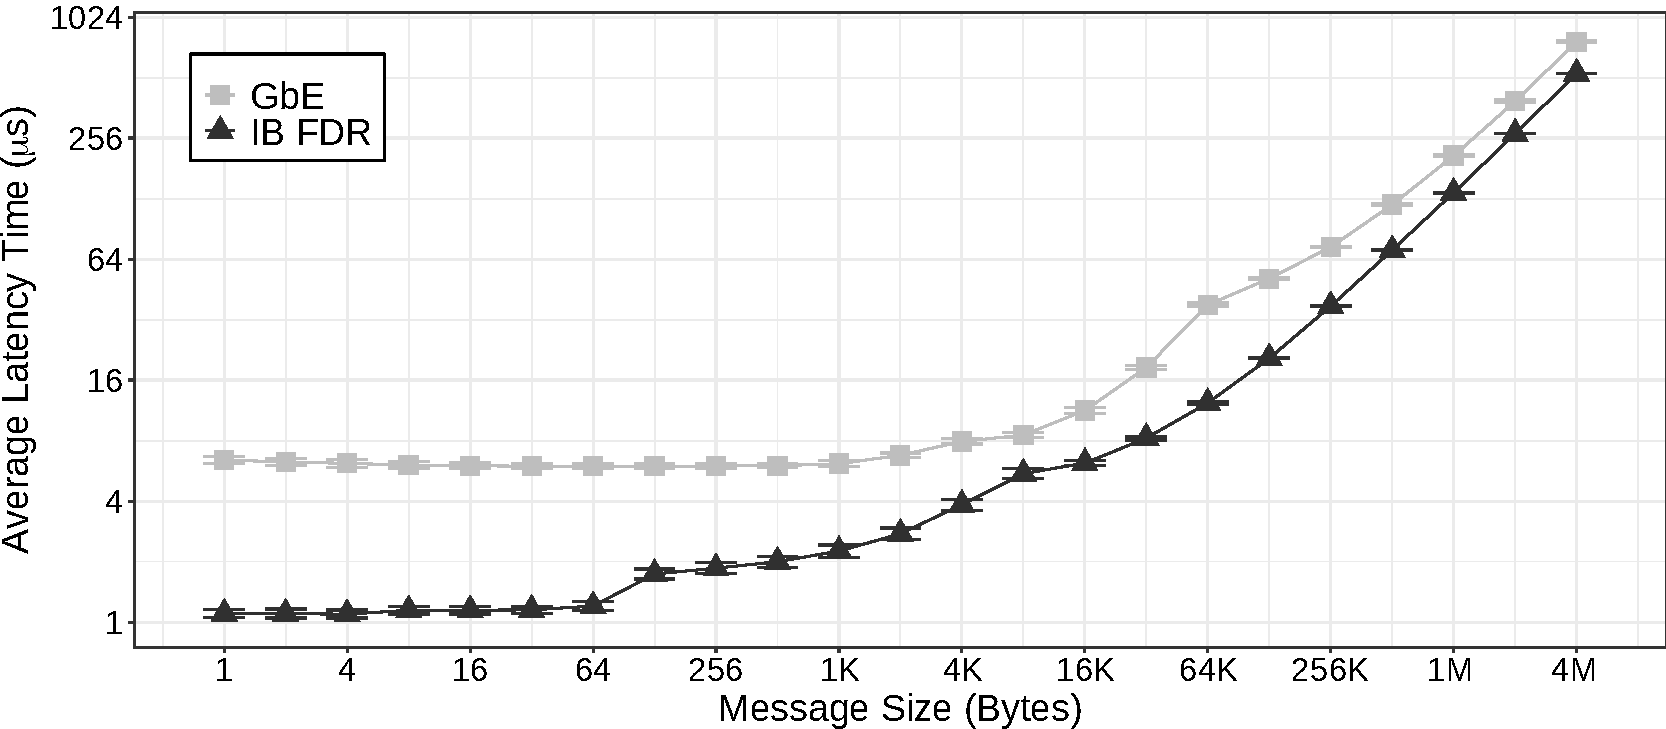
\includegraphics[width=\textwidth]{SLIDES/img/Latency.pdf}
\vfill\pause
\begin{itemize}
    \item InfiniBand latency is much lower\\
        $\to$ Similar results observed in the literature
    \item\pause IP-over-IB and Ethernet results overlap in all points\\
        $\to$ Non-observable performance differences
\end{itemize}
\end{frame}


\begin{frame}{Network Bandwidth}
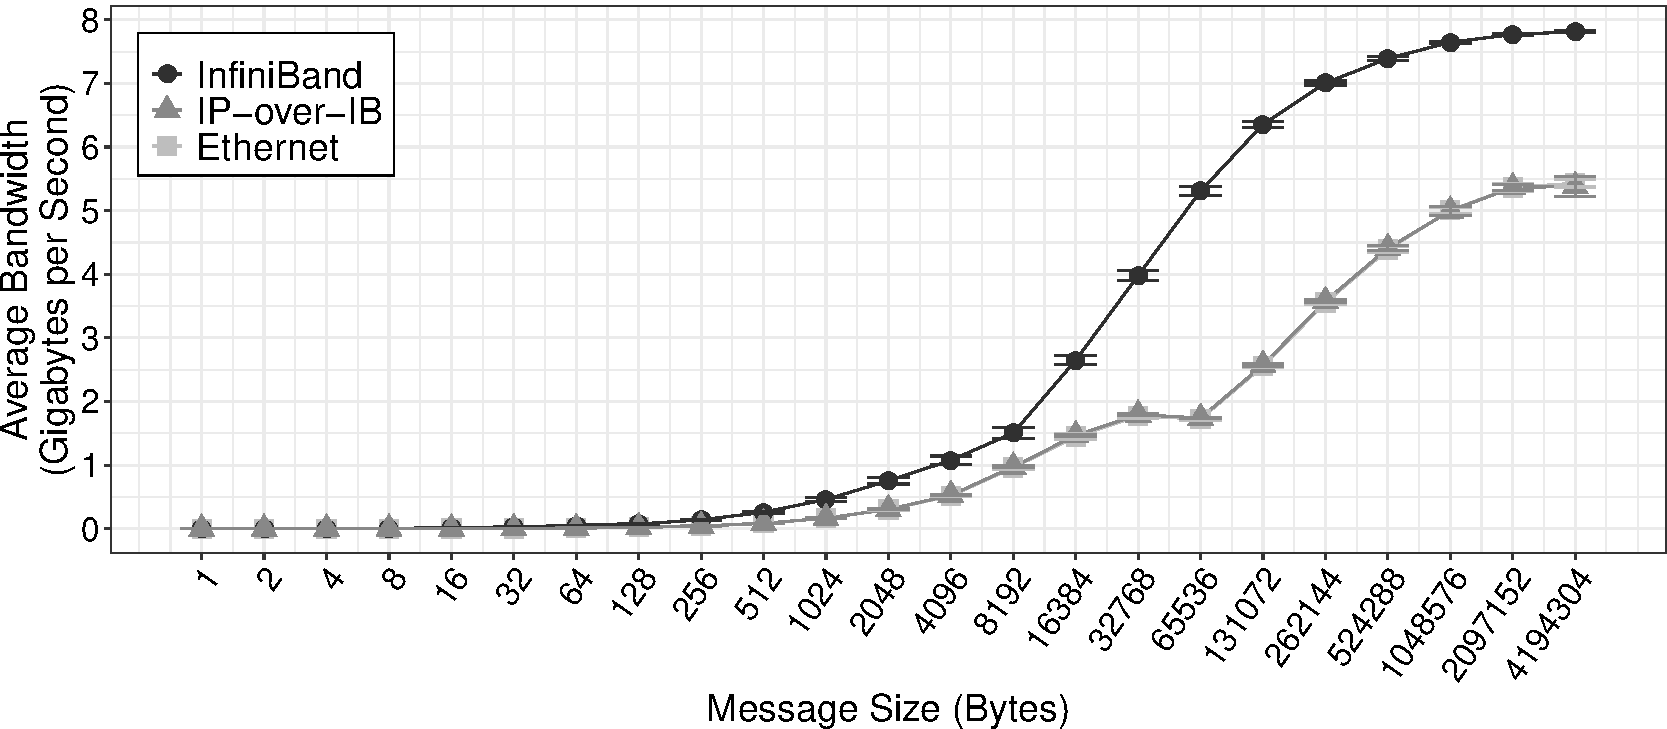
\includegraphics[width=\textwidth]{SLIDES/img/Bandwidth.pdf}
\vfill\pause
\begin{itemize}
    \item InfiniBand bandwidth starts to have a great difference since messages size with 8192 bytes\\
        $\to$ Similar results observed in the literature
    \item\pause Again, IP-over-IB and Ethernet results overlap in all points\\
        $\to$ Non-observable performance differences
\end{itemize}
\end{frame}

\begin{frame}{Analysis Of Interesting Cases (Execution Time)}
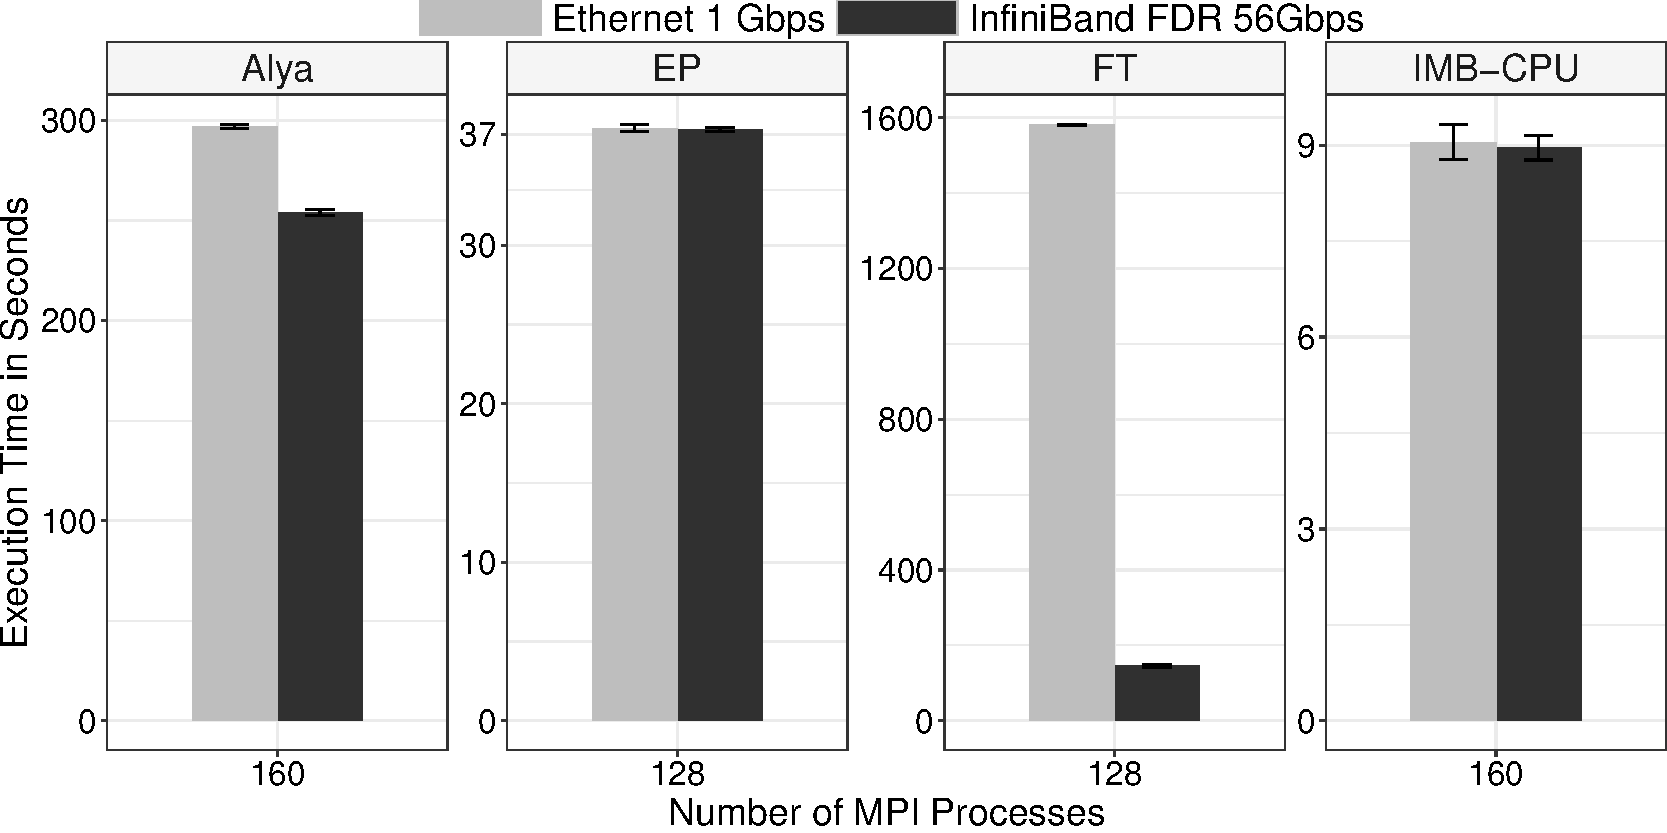
\includegraphics[width=\textwidth]{SLIDES/img/FT-EP-Alya-IMB.pdf}
Observations
\begin{itemize}
    \item teste
    \item teste
    \item item
\end{itemize}
\end{frame}

\begin{frame}{Analysis Of Interesting Cases (Execution Cost)}
\vspace{-1cm}
\begin{center}
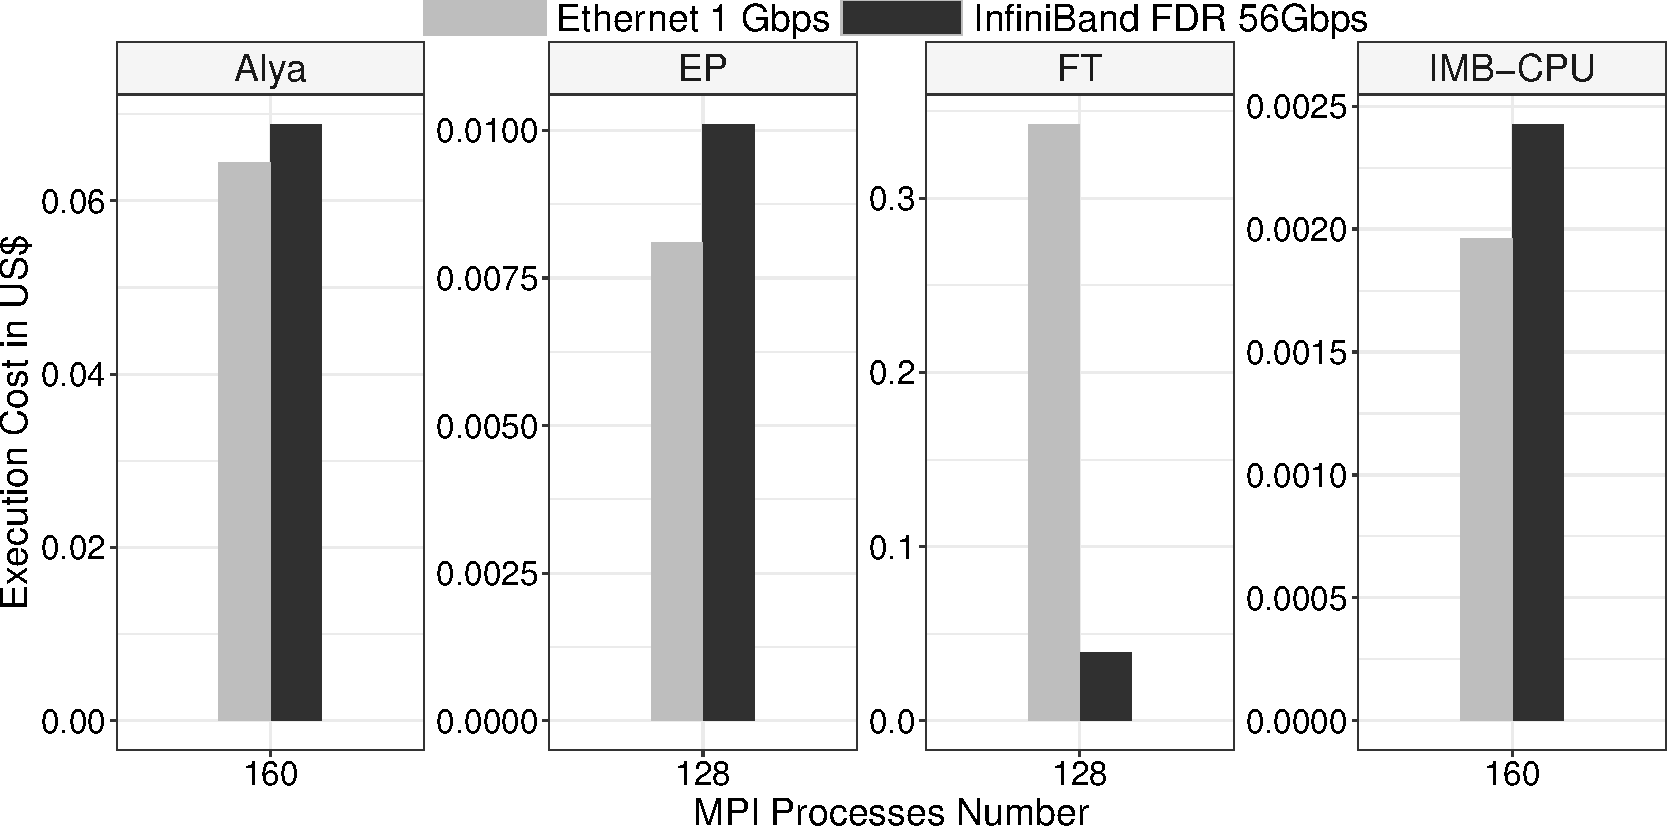
\includegraphics[scale=0.3]{SLIDES/img/FT-EP-Alya-IMB.cost.pdf}
\end{center}
\vspace{-0.5cm}
\begin{table}[h]
\resizebox{\textwidth}{!} \\
{\color[HTML]{000000} EP} & {\color[HTML]{000000} US\$ 0.03} & {\color[HTML]{000000} US\$ 0.04} & {\color[HTML]{000000} US\$ -0.01} & {\color[HTML]{000000} -19.81\%} \\
{\color[HTML]{000000} FT} & {\color[HTML]{000000} US\$ 1.36} & {\color[HTML]{000000} US\$ 0.16} & {\color[HTML]{000000} US\$ 1.21} & {\color[HTML]{000000} 770\%} \\
{\color[HTML]{000000} IMB-CPU} & {\color[HTML]{000000} US\$ 0.0078} & {\color[HTML]{000000} US\$ 0.0097} & {\color[HTML]{000000} US\$ -0.0019} & {\color[HTML]{000000} -19.59\%} \\ \hline
\end{tabular}%
}
\end{table}
\end{frame}

\begin{frame}{Analysis Of Interesting Cases (Characterization - Alya)}
\begin{figure}
   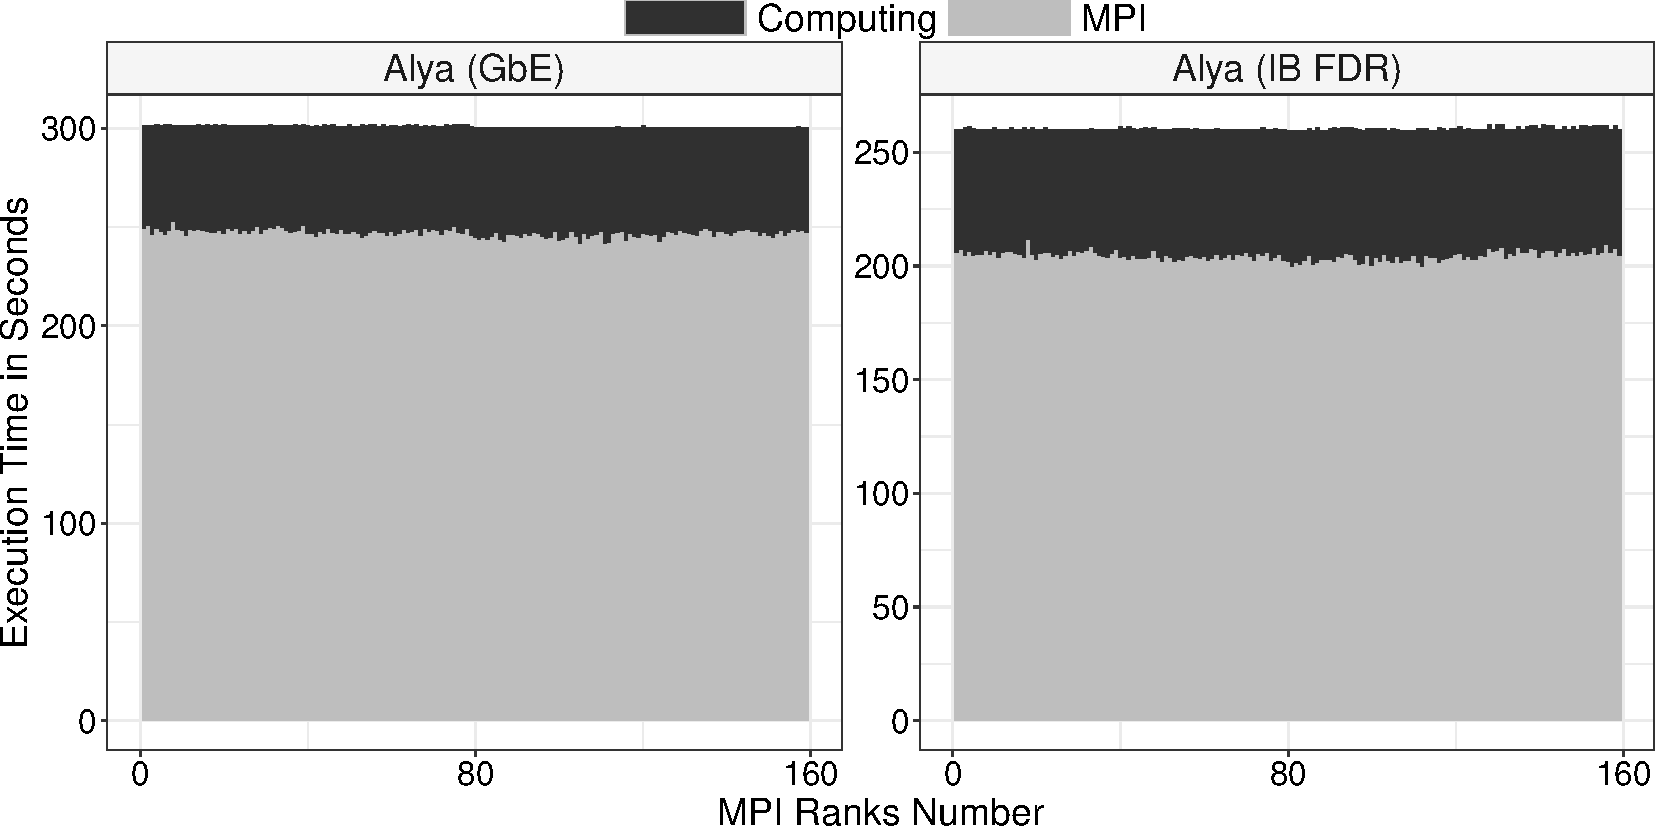
\includegraphics[width=0.61\textwidth]{SLIDES/img/Alya.charac.pdf}
   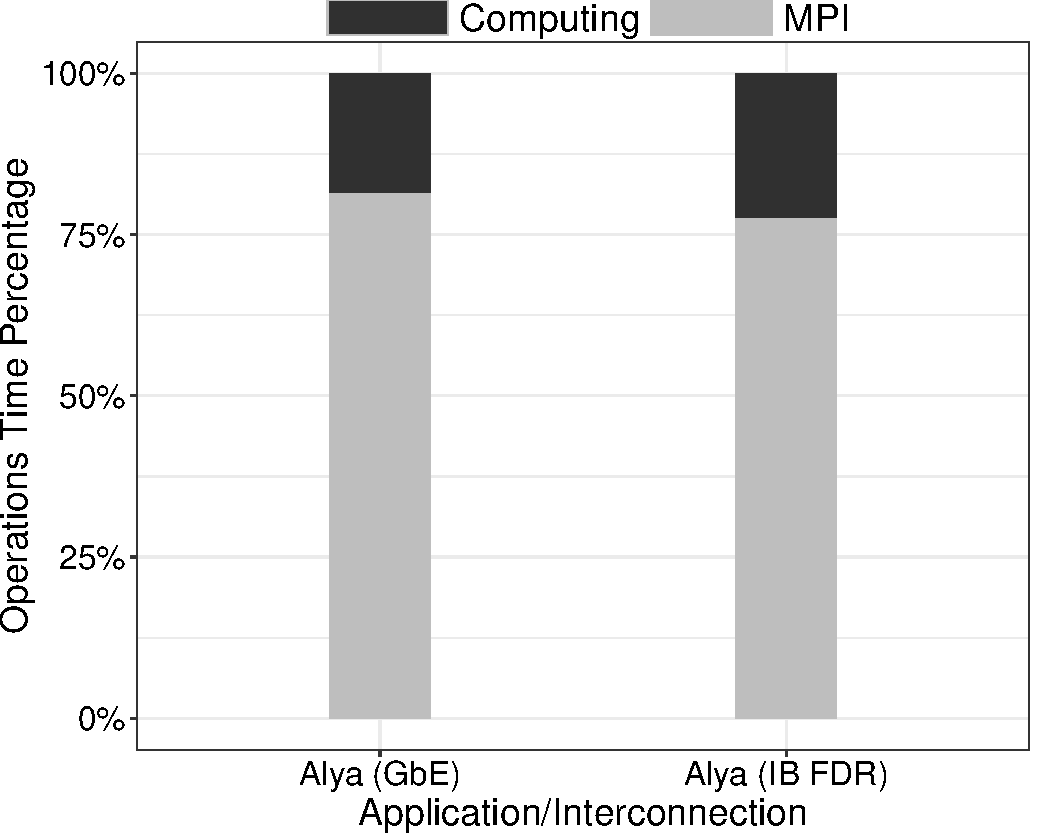
\includegraphics[width=0.38\textwidth]{SLIDES/img/Alya.percentage.pdf}
\end{figure}
Observations
\begin{itemize}
    \item teste
    \item teste
    \item item
    \item item
    \item teste
    \item teste
    \item teste
\end{itemize}
\end{frame}

\begin{frame}{Analysis Of Interesting Cases (Characterization - EP)}
\begin{figure}
   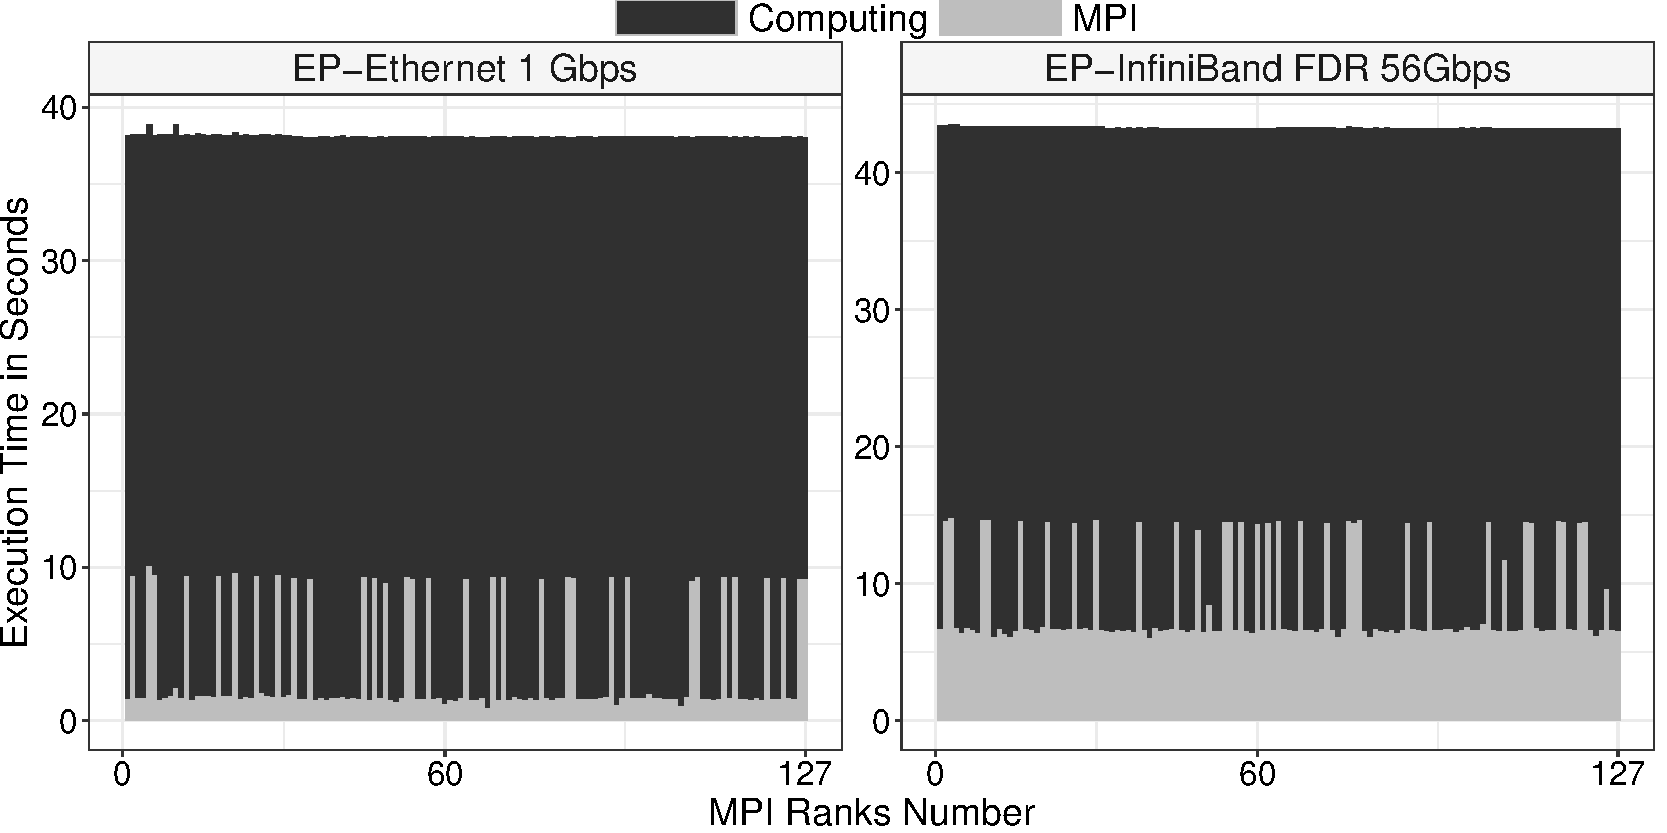
\includegraphics[width=0.61\textwidth]{SLIDES/img/EP.charac.pdf}
   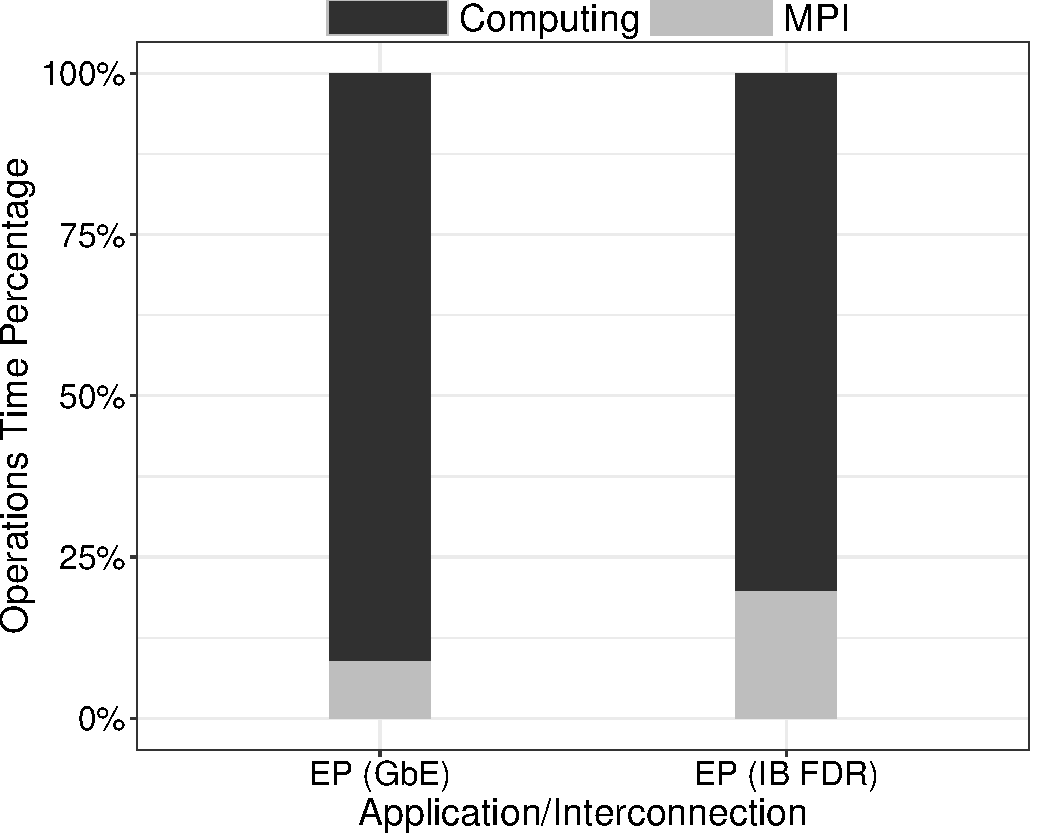
\includegraphics[width=0.38\textwidth]{SLIDES/img/EP.percentage.pdf}
\end{figure}
Observations
\begin{itemize}
    \item teste
    \item teste
    \item item
    \item item
    \item teste
    \item teste
    \item teste
\end{itemize}

\end{frame}

\begin{frame}{Analysis Of Interesting Cases (Characterization - FT)}
\begin{figure}
   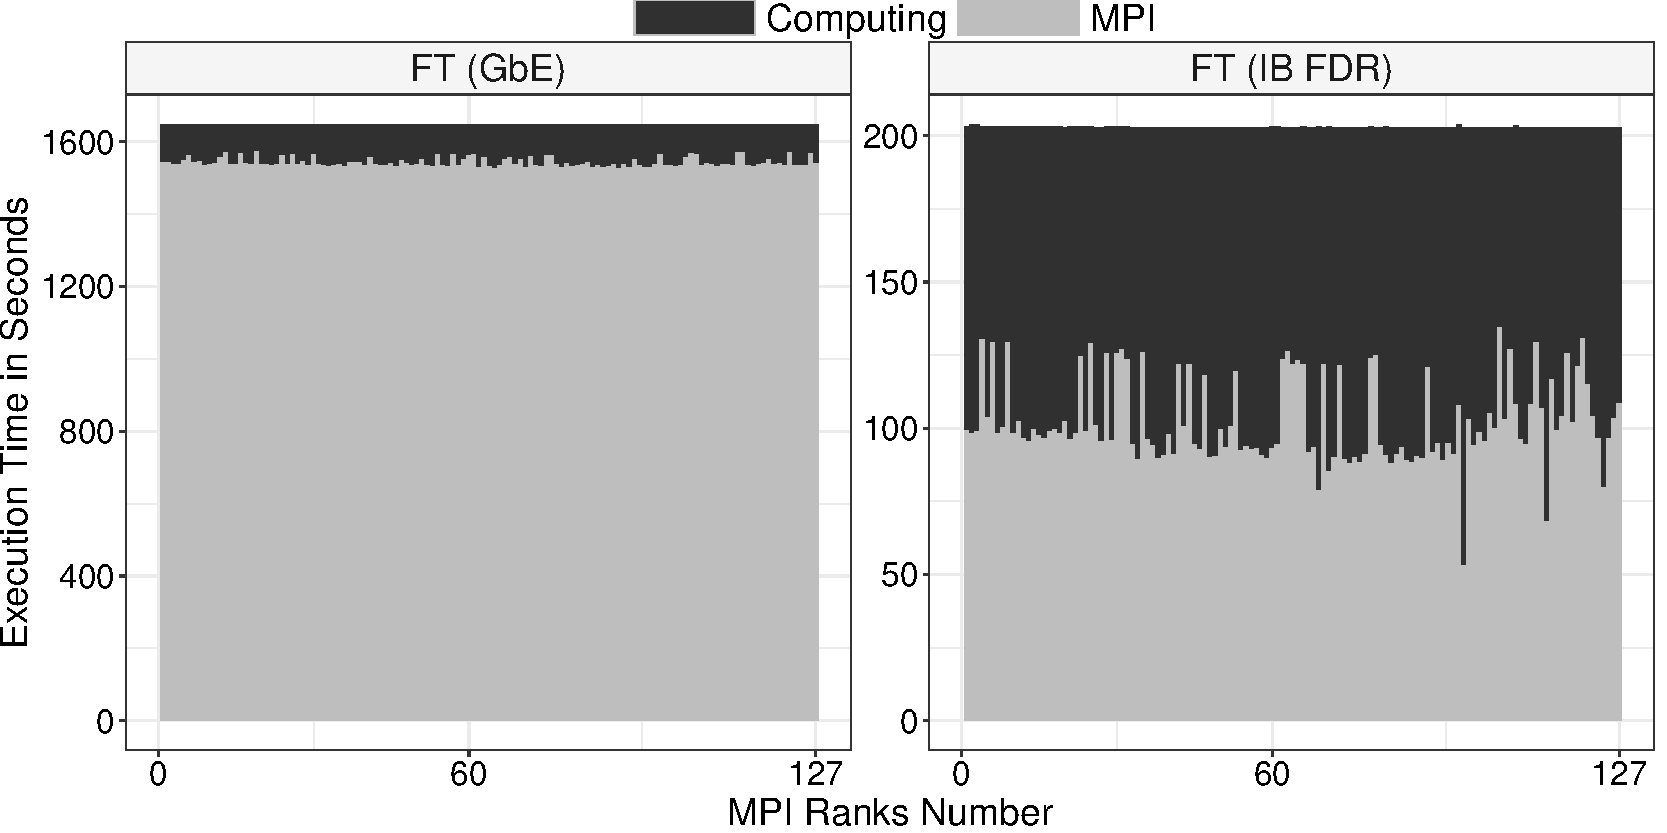
\includegraphics[width=0.61\textwidth]{SLIDES/img/FT.charac.pdf}
   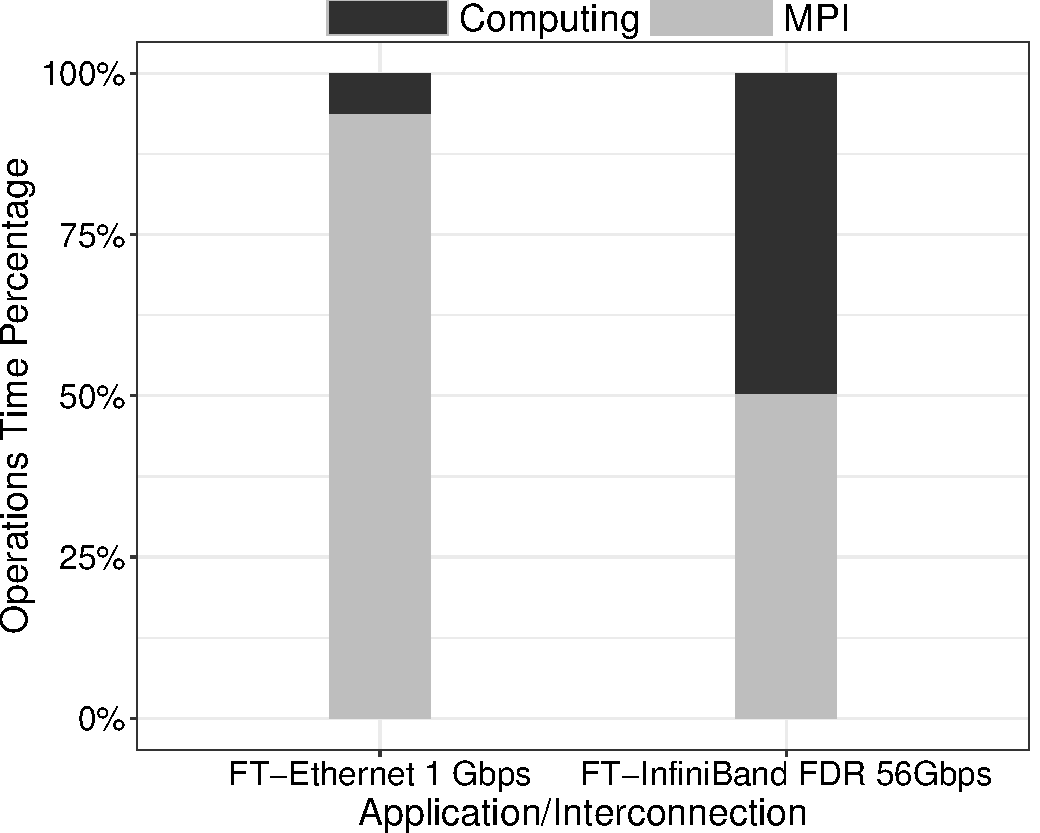
\includegraphics[width=0.38\textwidth]{SLIDES/img/FT.percentage.pdf}
\end{figure}
Observations
\begin{itemize}
    \item teste
    \item teste
    \item item
    \item item
    \item teste
    \item teste
    \item teste
\end{itemize}
\end{frame}

\begin{frame}{Analysis Of Interesting Cases (Characterization - IMB CPU)}
\begin{figure}
   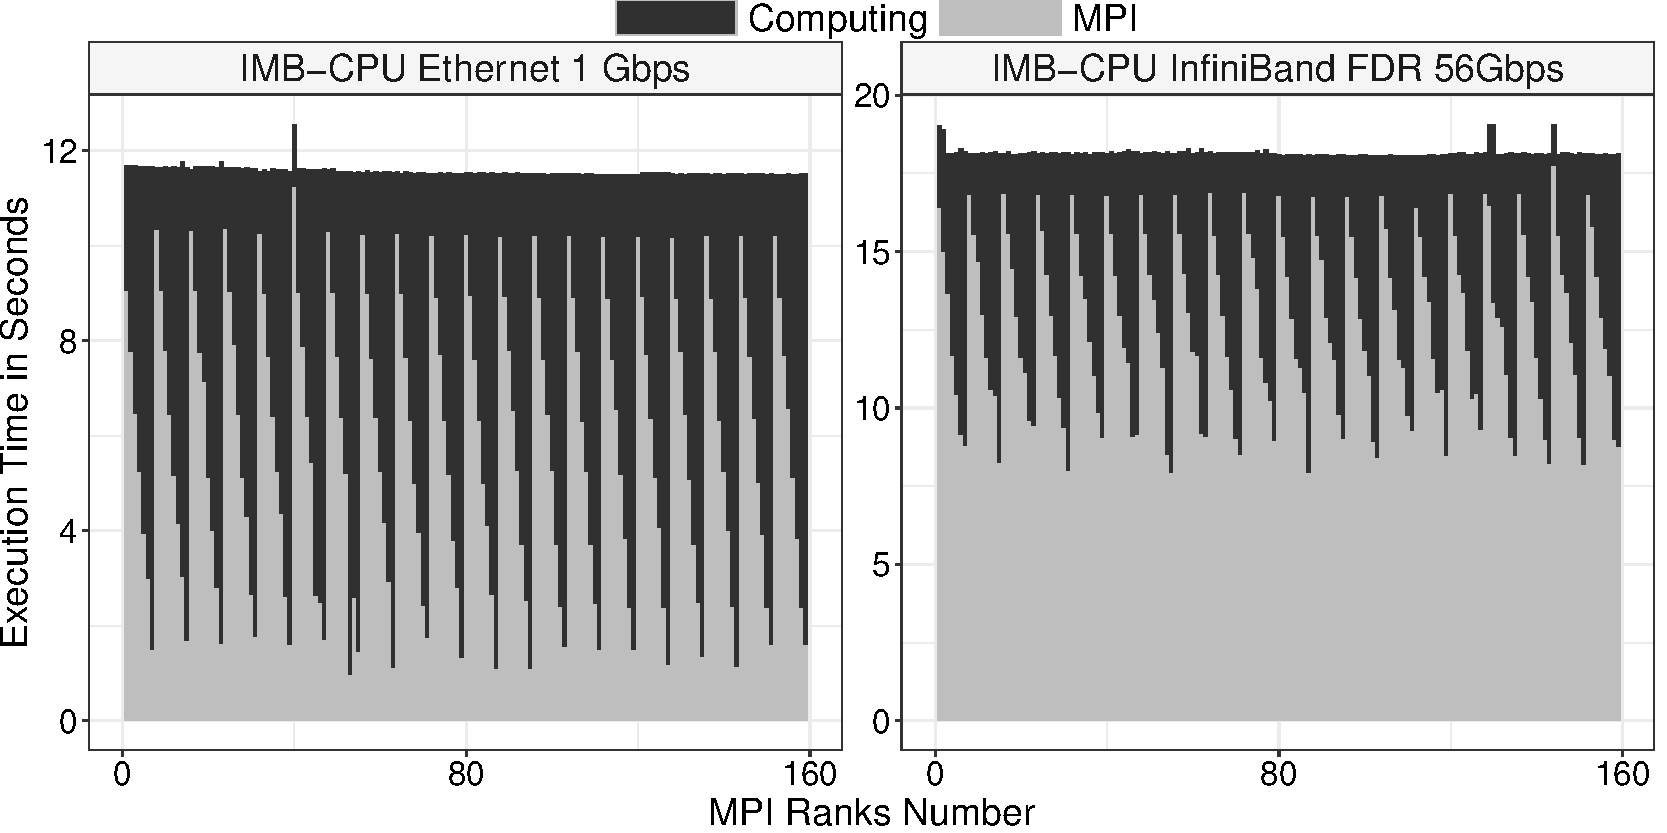
\includegraphics[width=0.61\textwidth]{SLIDES/img/IMB-CPU.charac.pdf}
   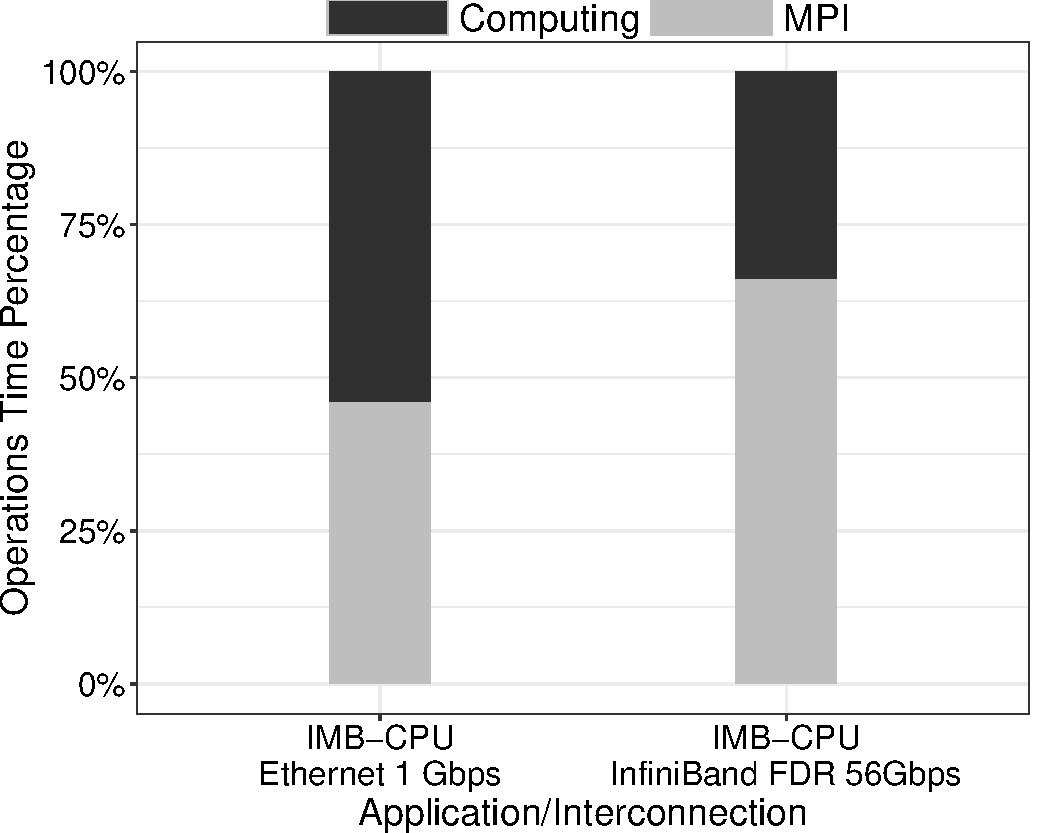
\includegraphics[width=0.38\textwidth]{SLIDES/img/IMB_CPU.percentage.pdf}
\end{figure}
Observations
\begin{itemize}
    \item teste
    \item teste
    \item item
    \item item
    \item teste
    \item teste
    \item teste
\end{itemize}
\end{frame}

\begin{frame}{Conclusion}

\end{frame}

\begin{frame}{References}

\end{frame}
\logo{}

\begin{frame}{}
\begin{center}
\Huge{Thank You!}
\vfill
\Large{ammaliszewski@inf.ufrgs.br}
\vfill
\small{https://github.com/andermm/CMP223.git}
\end{center}
\end{frame}

\logo{
\includegraphics[width=1.3cm,keepaspectratio]{SLIDES/logo/ufrgs.png}~~~~~~~~~~~~~~~~~~~~~~~~~~~~~~~~~~~~~~~~~~~~~~~~~~~~~~~~~~~~~~~~~~~~~
%\hspace{\dimexpr\paperwidth-5cm-1pt}%
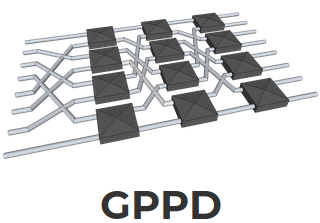
\includegraphics[width=1.3cm,keepaspectratio]{SLIDES/logo/GPPD-logo.png}~~~~~~~~~~~~~~~~~~~~~~~~~~~~~~~~~~~~~~~~~~~~~~~~~~~~~~~~~~~~~~~~~~~~~
%\hspace{\dimexpr\paperwidth-3cm-1pt}%

\includegraphics[width=1.5cm,keepaspectratio]{SLIDES/logo/inf-logo.png}%
}

\maketitle

\end{document}